\section{收敛与计算成本}
\label{sec:sqp-convergence}

各个部件都有了，本节回答三个问题：在解附近能收敛多快，什么时候算结束，以及每一轮的计算花在哪里。

\paragraph{精确Hessian的局部二次收敛}
先看只含等式的情形，记$\bm{w}=(\bm{x},\bm{\nu})$。定理~\ref{thm:sqp-newton}说全步长SQP就是$\bm{F}(\bm{w})=\bm{0}$上的Newton法，其Jacobian正是KKT矩阵$\bm{K}(\bm{w})$。所以收敛性的证明与第~\ref{chap:second-order-methods}章的证明思路相同，只是矩阵不再对称正定。

\begin{theorem}[SQP的局部二次收敛]
\label{thm:sqp-local-quadratic}
设$\bm{w}^\star=(\bm{x}^\star,\bm{\nu}^\star)$满足等式约束问题的KKT条件，$\bm{A}(\bm{x}^\star)$行满秩，并且$\nabla^2_{\bm{x}\bm{x}}\mathcal{L}(\bm{w}^\star)$在$\bm{A}(\bm{x}^\star)$的零空间上正定。设在半径为$r$的球内$\bm{K}$满足
\begin{equation}
 \lVert\bm{K}(\bm{w})-\bm{K}(\bm{w}')\rVert_2\leq M\lVert\bm{w}-\bm{w}'\rVert_2.
 \label{eq:sqp-k-lipschitz}
\end{equation}
令$\sigma>0$为$\bm{K}(\bm{w}^\star)$的最小奇异值。若$\lVert\bm{w}^{(t)}-\bm{w}^\star\rVert_2<\min\{r,\sigma/(2M)\}$，则全步长SQP的下一点有定义，且
\begin{equation}
 \lVert\bm{w}^{(t+1)}-\bm{w}^\star\rVert_2\leq\frac{M}{\sigma}\lVert\bm{w}^{(t)}-\bm{w}^\star\rVert_2^2.
 \label{eq:sqp-quadratic-bound}
\end{equation}
\end{theorem}

\begin{proof}
记$\bm{e}=\bm{w}^{(t)}-\bm{w}^\star$，$\bm{K}=\bm{K}(\bm{w}^{(t)})$。定理~\ref{thm:sqp-eqp}说明$\bm{K}(\bm{w}^\star)$可逆，所以$\sigma>0$。

第一步说明$\bm{K}$的逆有界。由式~\eqref{eq:sqp-k-lipschitz}，
\[
 \lVert\bm{K}-\bm{K}(\bm{w}^\star)\rVert_2\leq M\lVert\bm{e}\rVert_2\leq\frac\sigma2.
\]
最小奇异值的扰动不超过矩阵差的范数，所以$\bm{K}$的最小奇异值至少是$\sigma/2$，即
\[
 \lVert\bm{K}^{-1}\rVert_2\leq\frac2\sigma.
\]

第二步写出误差递推。由$\bm{F}(\bm{w}^\star)=\bm{0}$沿线段积分，
\[
 \bm{F}(\bm{w}^{(t)})=\int_0^1\bm{K}(\bm{w}^\star+s\bm{e})\bm{e}\,\mathrm{d}s.
\]

下一点是$\bm{w}^{(t)}$减去$\bm{K}^{-1}\bm{F}(\bm{w}^{(t)})$，把上式代入，得到
\[
 \bm{w}^{(t+1)}-\bm{w}^\star
 =\bm{K}^{-1}\int_0^1\bigl(\bm{K}-\bm{K}(\bm{w}^\star+s\bm{e})\bigr)\bm{e}\,\mathrm{d}s.
\]

第三步估计积分。由式~\eqref{eq:sqp-k-lipschitz}，被积函数的范数不超过$M(1-s)\lVert\bm{e}\rVert_2^2$，积分后得
\[
 \Bigl\lVert\int_0^1\bigl(\bm{K}-\bm{K}(\bm{w}^\star+s\bm{e})\bigr)\bm{e}\,\mathrm{d}s\Bigr\rVert_2\leq\frac M2\lVert\bm{e}\rVert_2^2.
\]
再乘以第一步的界，式~\eqref{eq:sqp-quadratic-bound}成立。
\end{proof}

这里$M$是$\bm{K}$的Lipschitz常数，它由$f$与$h_j$的三阶导数大小和乘子的大小共同决定，当目标和约束的Hessian都Lipschitz连续时存在。由于$\lVert\bm{e}\rVert_2<\sigma/(2M)$时式~\eqref{eq:sqp-quadratic-bound}的右端小于$\lVert\bm{e}\rVert_2/2$，迭代留在球内，二次收敛一直保持。

条件各有用处。行满秩和约化曲率正定都是用来保证$\bm{K}(\bm{w}^\star)$可逆的，这正是定理~\ref{thm:sqp-eqp}的条件。注意结论是关于$\bm{w}$的。单看$\bm{x}$的误差，或单看违反量，不必单调下降，表~\ref{tab:sqp-newton-run}中$t=1$到$t=2$的$\lvert h\rvert$就几乎不动。

\paragraph{含不等式时}
由定理~\ref{thm:sqp-identification}，LICQ、严格互补和二阶充分条件下，靠近解时局部QP有一个活动集恰为$\bm{S}^\star$的解。若求解器返回这个解，SQP就和把$\bm{S}^\star$当作等式的SQP完全一样，定理~\ref{thm:sqp-local-quadratic}适用于这个等式问题，得到二次收敛。

这里有三个“若”，缺一不可：活动集已被识别，全步长被接受，并且QP求解器选中了这个解。第二点正是上一节二阶修正要保证的。

\paragraph{拟Newton的局部超线性收敛}
用近似矩阵时，分析更细。在同样的约束资格和二阶充分条件下，若迭代已收敛于解、步长为$1$，并且$\bm{B}^{(t)}$有界，式~\eqref{eq:sqp-dennis-more}是$\bm{x}^{(t)}$超线性收敛的刻画。这个结论的证明要比较拟Newton步与精确Newton步的差，篇幅较长，读者可查阅专著\scite{math-nocedal2006numerical}。

条件不会自动成立。全空间的BFGS矩阵需要沿$\bm{d}^{(t)}$的切向分量持续得到好的曲率信息，阻尼会使一部分更新偏离割线条件。已知的保证多是两步超线性这样较弱的形式，或者依赖额外的假设。图~\ref{fig:sqp-exact-bfgs-rate}中尾部的快速下降是一次运行的现象，不能当作普遍定理。

\paragraph{远离解时}
上面的结论都假定初始点已经足够接近解。远离解时依靠接受规则。对罚函数线搜索，常见的全局结论是：若迭代点留在紧集内，$f,g_i,h_j$足够光滑，约束梯度在其上一致线性无关，$\bm{B}^{(t)}$一致有界且一致正定，$\rho$最终固定下来，QP都相容，则极限点是原问题的KKT点。证明要用到式~\eqref{eq:sqp-merit-descent}给出的逐步下降以及回溯的步长下界，读者可查阅专著\scite{math-nocedal2006numerical}。过滤器有相应的结论，需要它自己的一组假设。

这种结论要求的条件不同于局部结论，得到的也只是KKT点，不是全局最优解，非凸问题上它可能收敛到鞍点甚至极大方向的驻点附近。图~\ref{fig:sqp-global-local}是问题~\eqref{eq:sqp-circle}从远处出发的运行。圆上还有另一个KKT点$(-1,-1)^\top$，那是圆上目标的最大点，乘子$\nu=-1/2$，起点$(0.2,-1.6)^\top$在圆的下方。

\begin{BookInlineFigure}
 \centering
 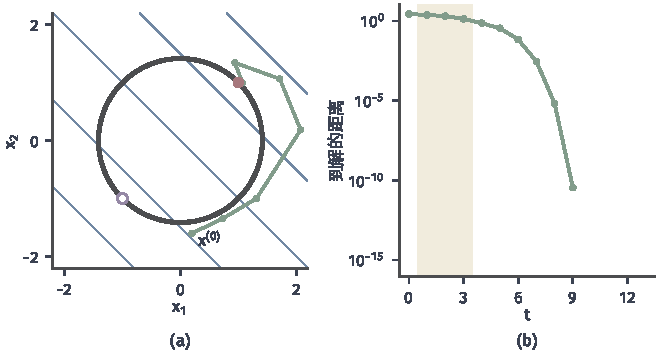
\includegraphics[width=112mm]{figures/05-optimization/06-constrained-optimization/matplotlib/sqp-global-local/figure.pdf}
 \caption{问题~\eqref{eq:sqp-circle}从$(0.2,-1.6)^\top$、$\nu^{(0)}=1$出发的回溯SQP，$\rho=1$，约化曲率不足$0.5$时移位。(a)~路径（绿）绕过圆的右侧到达解（红点），紫色空心点是圆上目标的最大点。(b)~到解的距离，黄色带是步长小于$1$的轮次，此后全步长二次收敛。}
 \label{fig:sqp-global-local}
\end{BookInlineFigure}

运行分成两个阶段。前四轮步长依次是$1,0.25,0.5,0.5$，其中第二到第五轮的约化曲率不足，加了移位，这是接受规则和曲率修正在起作用。之后步长一直是$1$，到解的距离依次为$0.347$、$0.0686$、$0.00289$、$6.7\times10^{-6}$、$3.5\times10^{-11}$，进入Newton的快速段。

\paragraph{停止准则}
“QP解完了”不是结束的标志，判断要回到原问题的KKT残差上。给定容差$\varepsilon_{\mathrm{p}},\varepsilon_{\mathrm{d}},\varepsilon_{\mathrm{c}}>0$，同时检查原始可行、Lagrange驻定和互补三项：
\begin{equation}
 \begin{gathered}
 \lVert\bm{h}(\bm{x})\rVert_\infty\leq\varepsilon_{\mathrm{p}},\qquad\lVert[\bm{g}(\bm{x})]_+\rVert_\infty\leq\varepsilon_{\mathrm{p}},\\
 \lVert\nabla f(\bm{x})+\bm{A}^\top\bm{\nu}+\bm{G}^\top\bm{\lambda}\rVert_\infty\leq\varepsilon_{\mathrm{d}},\\
 \bm{\lambda}\geq\bm{0},\qquad\max_i\lvert\lambda_ig_i(\bm{x})\rvert\leq\varepsilon_{\mathrm{c}}.
 \end{gathered}
 \label{eq:sqp-stopping}
\end{equation}
三项的单位不同，实际中要按目标与约束的尺度归一化。步长很小不能作为收敛的证据，那可能只是回溯失败。

\paragraph{一轮的成本}
表~\ref{tab:sqp-cost}按$n$个变量、$p+m$条约束的稠密情形列出一轮的主要开销。其中QP的迭代次数$k$在热启动的后期常常是$1$或很小的数，而在早期、活动集变动频繁时可能很大。

\begin{BookInlineTable}
 \centering
 \begin{tabular}{ll}
  \toprule
  项目 & 开销\\
  \midrule
  一阶导数 & $\nabla f$与$\bm{A},\bm{G}$各一次\\
  精确曲率 & $m+p+1$个Hessian或Hessian向量积\\
  拟Newton更新 & 约$O(n^2)$\\
  KKT分解（等式） & 约$O((n+p)^3)$，稀疏时远小于此\\
  工作集迭代 & $k$次，每次低秩修正约$O(n^2)$\\
  步的接受 & 每次试探$f$和约束各一次\\
  二阶修正 & 约束一次，再加一次回代\\
  恢复阶段 & 额外的模型构造与子问题求解\\
  \bottomrule
 \end{tabular}
 \caption{SQP一轮的主要开销。}
 \label{tab:sqp-cost}
\end{BookInlineTable}

和第~\ref{chap:penalty-multiplier-methods}章的方法相比，SQP每轮贵得多，一轮要解一个QP，但轮数通常很少，适合函数求值昂贵、约束数目不太大的问题。约束和变量都很多、活动集又难以确定时，分解和工作集迭代的开销变大，第~\ref{chap:nonlinear-interior-point}章的内点法每轮结构更固定，往往更合适。
